\documentclass{article}
\usepackage[portrait, margin=1in]{geometry}
\usepackage{graphicx} 
\graphicspath{{/Users/danpost/consumer_sentiment/output/umich_figures/gaspx}{/Users/danpost/consumer_sentiment/output/umich_figures/macro_vars}}
\usepackage{amsmath}
\usepackage{hyperref}
\usepackage{threeparttable}
\usepackage{subcaption}

\title{University of Michigan's Surveys of Consumers Respondents' Sensitivity to Macroeconomic Conditions}
\author{Daniel Posthumus}

\begin{document}

\maketitle

\section{Introduction}

We know that Republicans and Democrats experience the economy very differently, depending on whether the White House is occupied by a President of their party or not. Previous \href{https://www.briefingbook.info/p/asymmetric-amplification-and-the}{research} by Cummings and Mahoney has shown this bias to be \textit{asymmetric}, with Republicans' partisan bias estimated to be two and a half times larger than Democrats'.

We can go beyond breaking down the top-line consumer sentiment index by partisan affiliation: the University of Michigan's Surveys of Consumers asks respondents about a host of different areas of the economy and their attitudes, not all of which are directly used in the calculation of the headline index. Starting in 2017, we can therefore re-create an aggregate measure of respondents' attitudes towards specific parts of the economy, split up by party.\footnote{The Survey only started to ask about respondents' partisan affiliation in 2017.} Using individual-level microdata, for example, we can calculate respondents' net attitudes ((\% who have a positive attitude) - (\% who have a negative attitude) + 100) by partisan affiliation, e.g. for personal financial conditions and broad business conditions. 

These descriptives, as we'll demonstrate, motivate an analysis of the association between observed economic variables and what people feel about the economy--and comparing these sensitivities between Democrats, Republicans, and Independents. At a high level, we regress changes in economic conditions on respondents' attitudes towards those specific factors--running a separate regression for whether Biden is president or not, as well as separate regressions for each partisan affiliation. One can thus think of the intercept in this model as indicating a partisan pre-set bias that varies by who is President and the slope term as respondents' sensitivity to the changing economy. What we find matches Cummings and Mahoney's previous findings: Republicans consistently display the strongest biases in formulating their attitudes towards the economy. 

\section{Motivation - Descriptive Evidence of Partisan Bias}

We know that voters' ideas about the economy are not a direct result of observed economic conditions; instead, voters filter their beliefs about the economy through attitudes towards government economic policy, which is in turn shaped by the partisan identity of the president. As the graphs below suggest, Republicans and Democrats reversed their respective attitudes towards government economic policy and--with some parallel shifts because of COVID and later inflationary dynamics--also towards both personal and broad economic conditions nearly exactly when Joe Biden took office.\footnote{The moving average smoothing makes this switch look much less drastic than the raw data suggests.}

%%%%%%%%%%%%%%%%%%%%%%%%%%%%%%%%%%%%%%%%%%%%%%%%%%%%%%%%%%%%%%%%%%%%%%%%%%%%%%%%%%%%
% govt/bago/pago panel of time-series
\begin{figure}[ht!]
  \centering
  \begin{subfigure}[b]{0.49\textwidth}
    \centering
    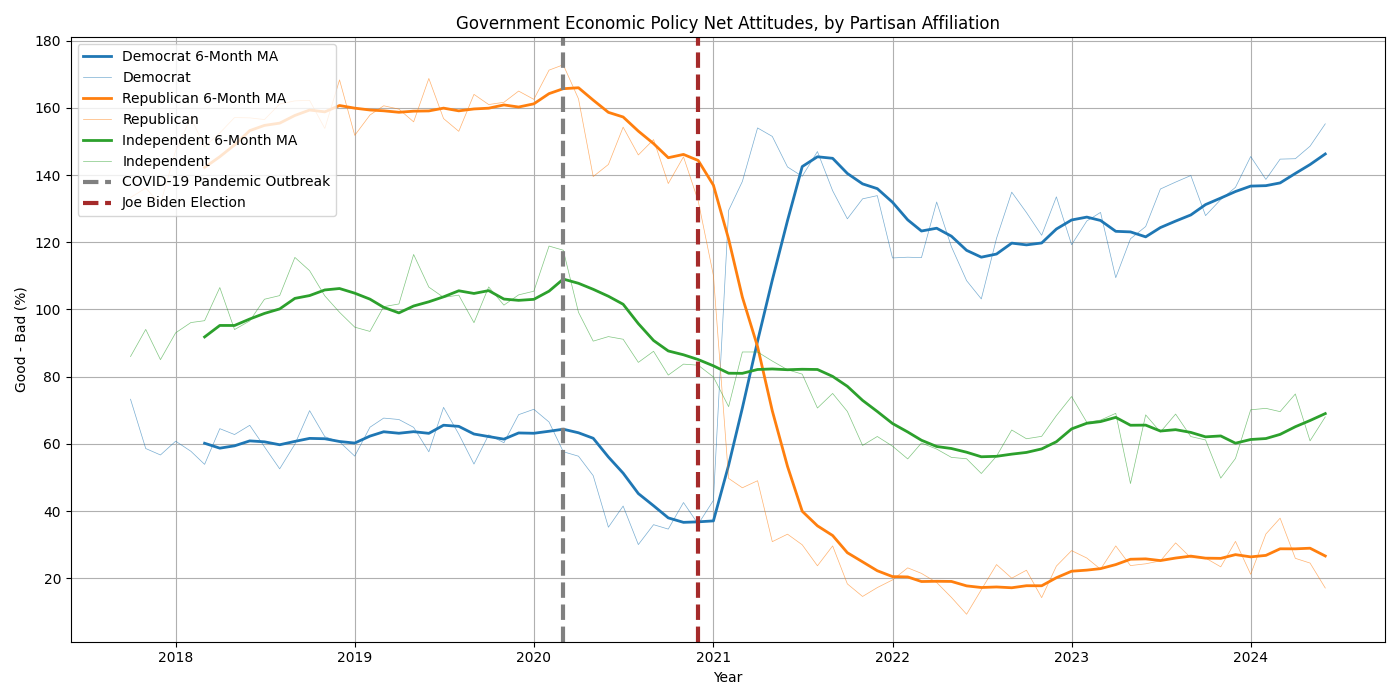
\includegraphics[width=\textwidth]{govt_r_time_series.png}
   % \caption{Government Economic Policy}
    \label{fig:govt_time_series}
  \end{subfigure}
  \begin{subfigure}[b]{0.49\textwidth}
    \centering
    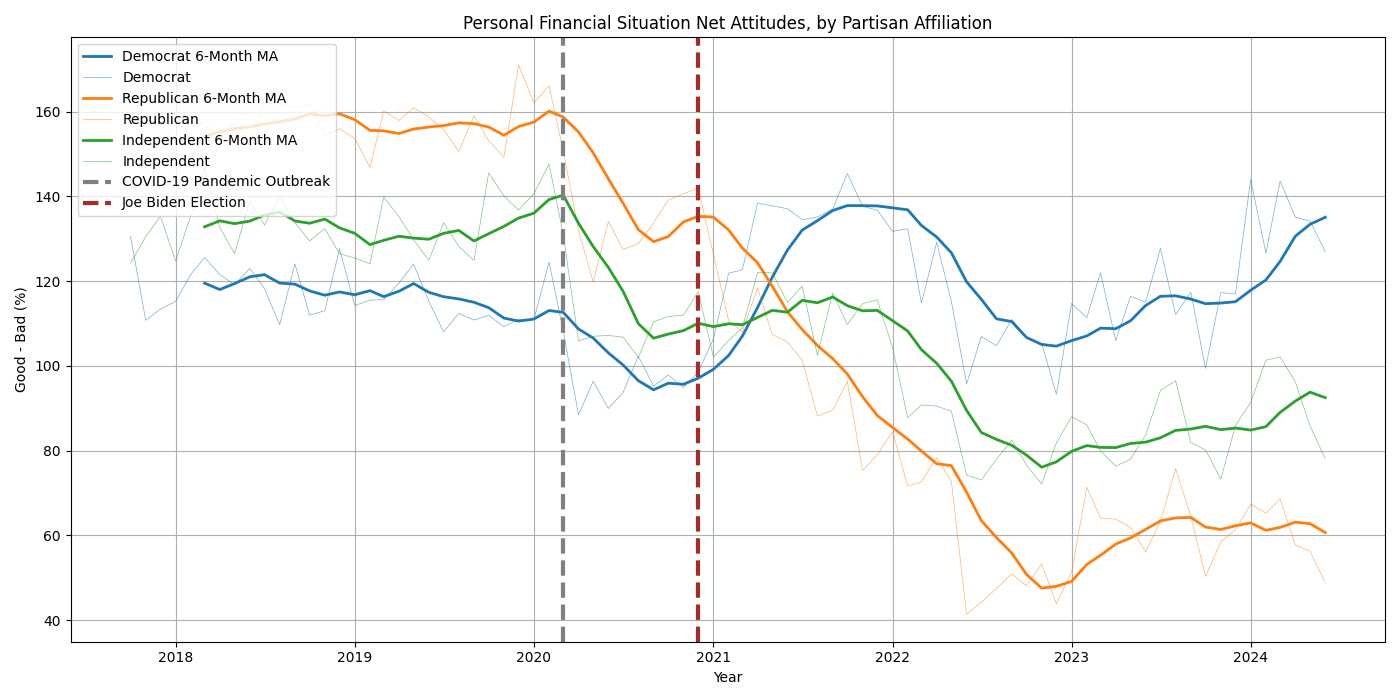
\includegraphics[width=\textwidth]{pago_r_time_series.png}
   % \caption{Personal Financial Conditions}
    \label{fig:pago_time_series}
  \end{subfigure}
   \begin{subfigure}[b]{0.5\textwidth}
    \centering
    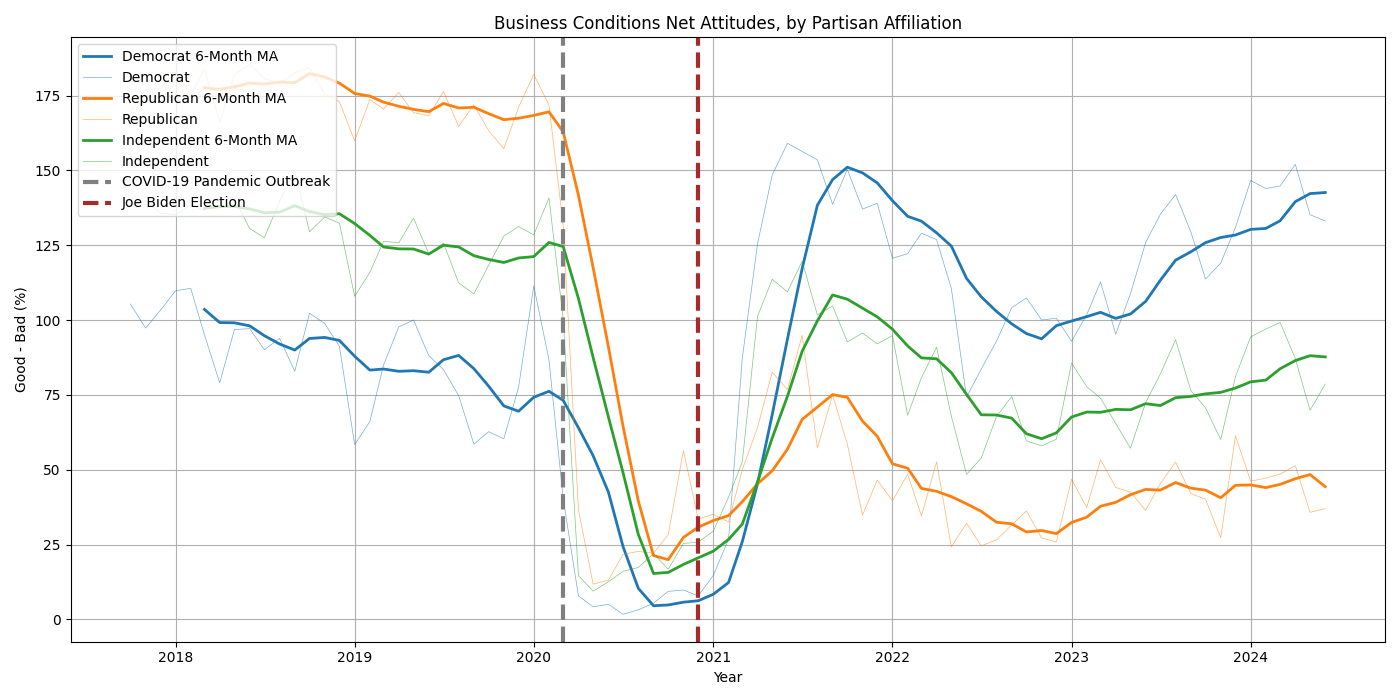
\includegraphics[width=\textwidth]{bago_r_time_series.png}
    %\caption{Broad Business Conditions}
    \label{fig:bago_time_series}
  \end{subfigure}
  \caption{Reconstructed Net Attitudes by Partisan Affiliation}
  \label{fig:panel}
\end{figure}

These are broad variables; there is no single indicator we can match them to. On the other hand, there is a clear indicator we can point to when it comes to gas prices, home value, inflation, or the stock market. Additionally, respondents of either political stripe are clearly not entirely immune to observed economic conditions: Republicans attitudes towards broad business conditions tanked under the Trump administration and subsequently improved under the Biden administration, presumably because of the COVID shock and recovery. So, we can take a closer look at specific parts of the economy by reconstructing this net attitude for specific questions: 

%%%%%%%%%%%%%%%%%%%%%%%%%%%%%%%%%%%%%%%%%%%%%%%%%%%%%%%%%%%%%%%%%%%%%%%%%%%%%%%%%%%%
% gas1/news_u_pri/hom/rinc/car/pstk panel of time-series
\begin{figure}[ht!]
  \centering
  \begin{subfigure}[b]{0.49\textwidth}
    \centering
    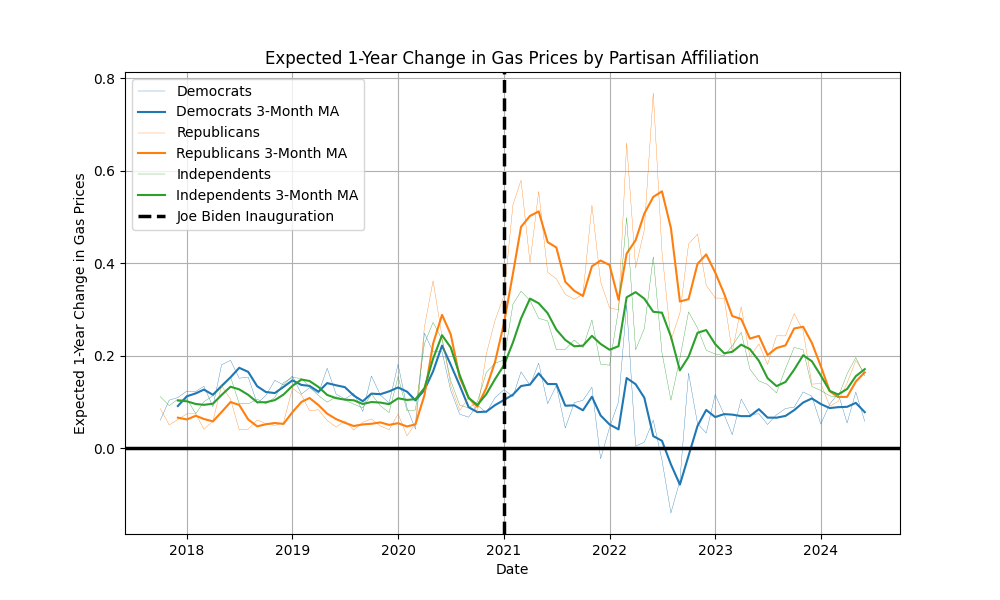
\includegraphics[width=\textwidth]{gas1_party_comp.png}
    %\caption{Predicted 1-Year Change in Gas Prices}
    \label{fig:gas1_time_series}
  \end{subfigure}
  \begin{subfigure}[b]{0.49\textwidth}
    \centering
    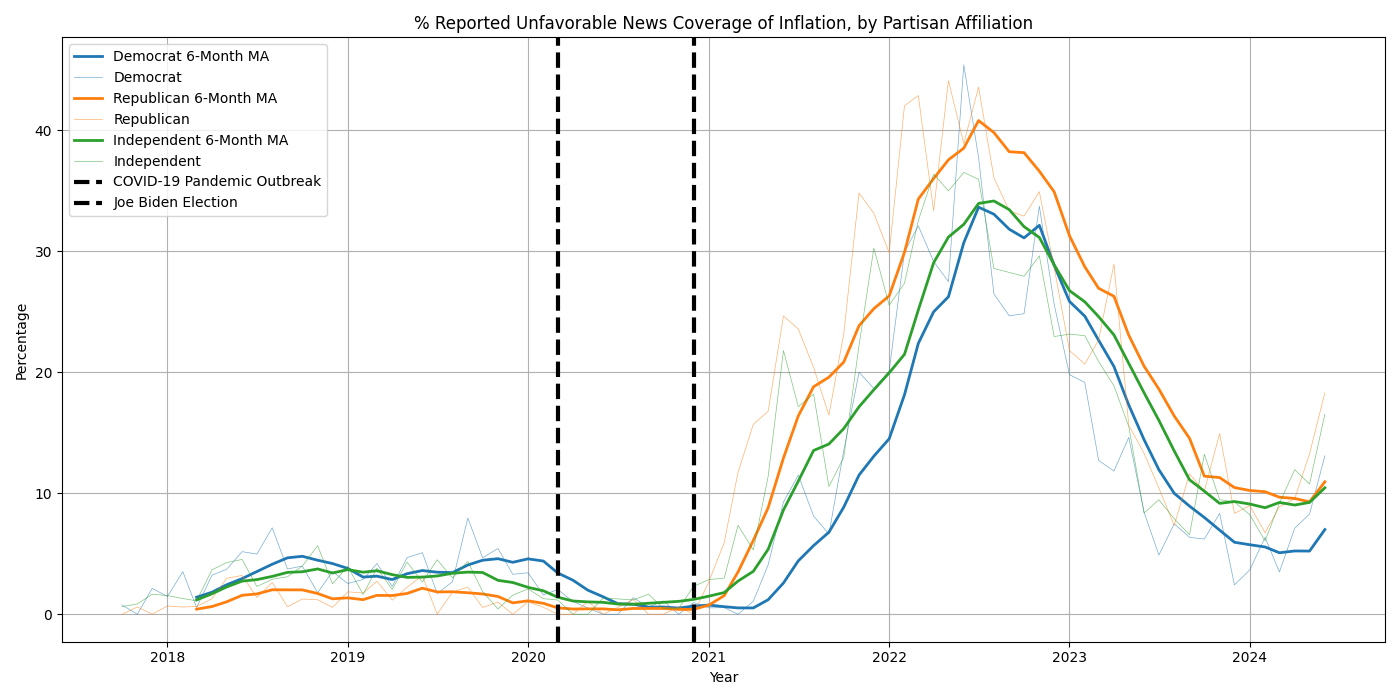
\includegraphics[width=\textwidth]{newsrn_u_pri_time_series.png}
   % \caption{Reported Unfavorable News Coverage of Inflation}
    \label{fig:newsrn_u_pri_time_series}
  \end{subfigure}
   \begin{subfigure}[b]{0.49\textwidth}
    \centering
    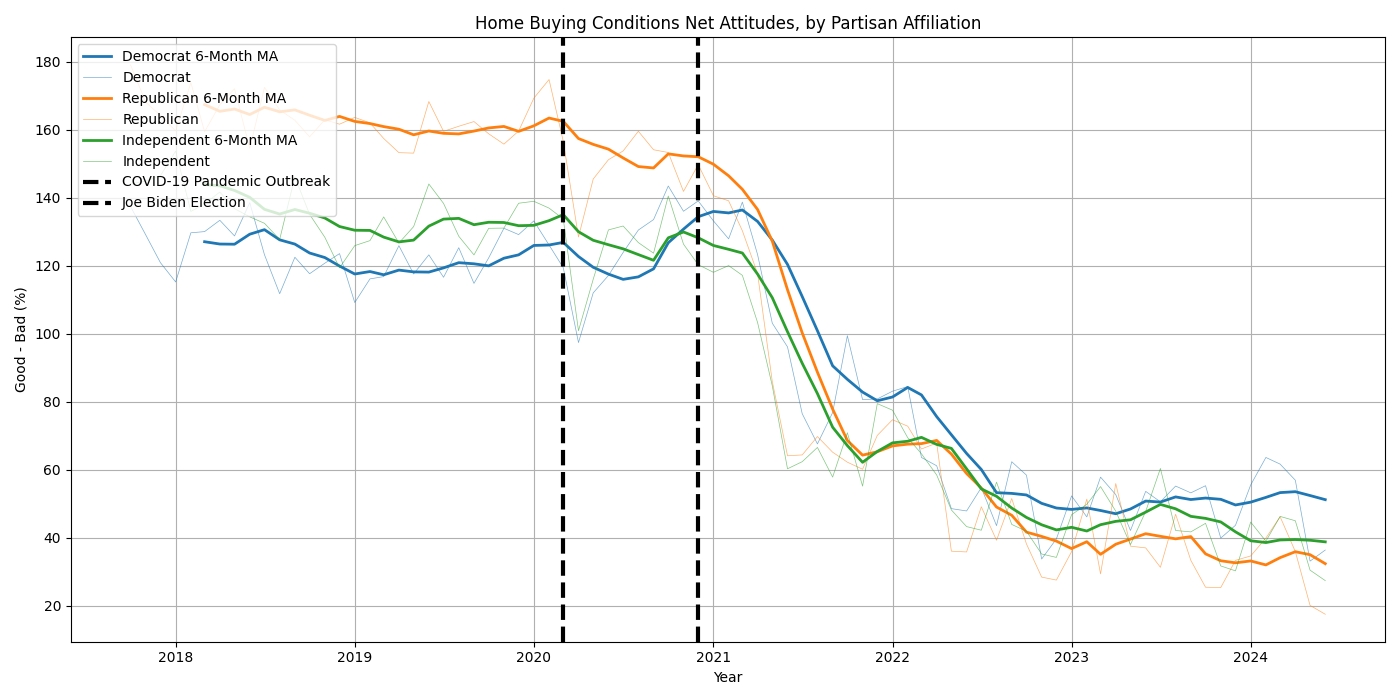
\includegraphics[width=\textwidth]{hom_r_time_series.png}
    %\caption{Home-Buying Conditions}
    \label{fig:hom_time_series}
  \end{subfigure}
   \begin{subfigure}[b]{0.49\textwidth}
    \centering
    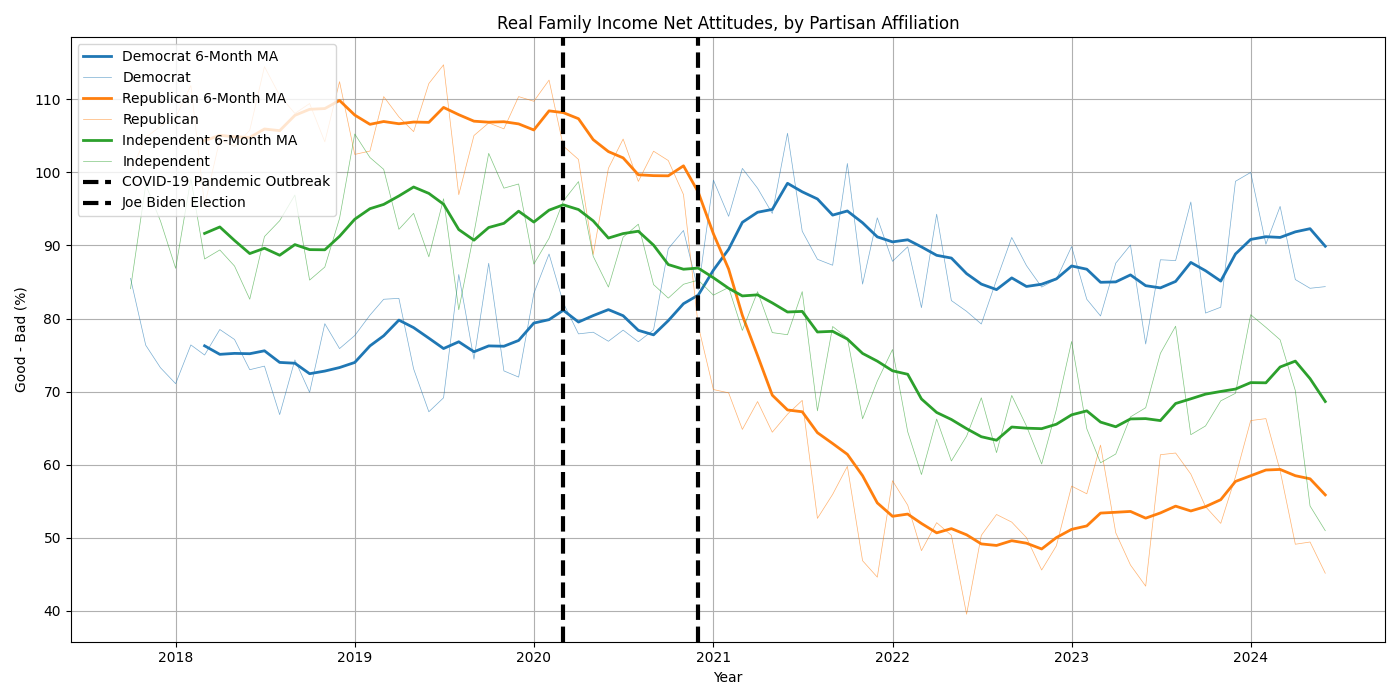
\includegraphics[width=\textwidth]{rinc_r_time_series.png}
    %\caption{Real Household Income}
    \label{fig:rinc_time_series}
  \end{subfigure}
   \begin{subfigure}[b]{0.49\textwidth}
    \centering
    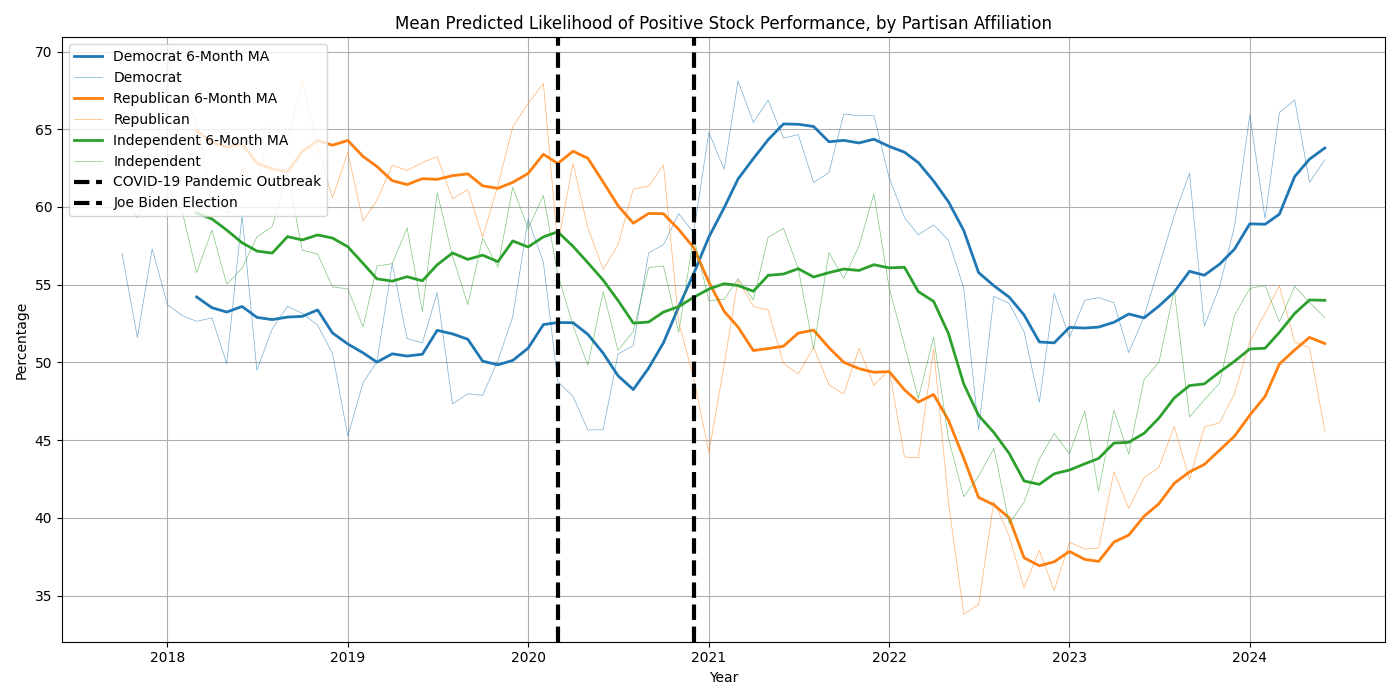
\includegraphics[width=\textwidth]{PSTK_time_series.png}
    %\caption{Predicted Likelihood of Positive Stock Market Return}
    \label{fig:pstk_time_series}
  \end{subfigure}
   \begin{subfigure}[b]{0.49\textwidth}
    \centering
    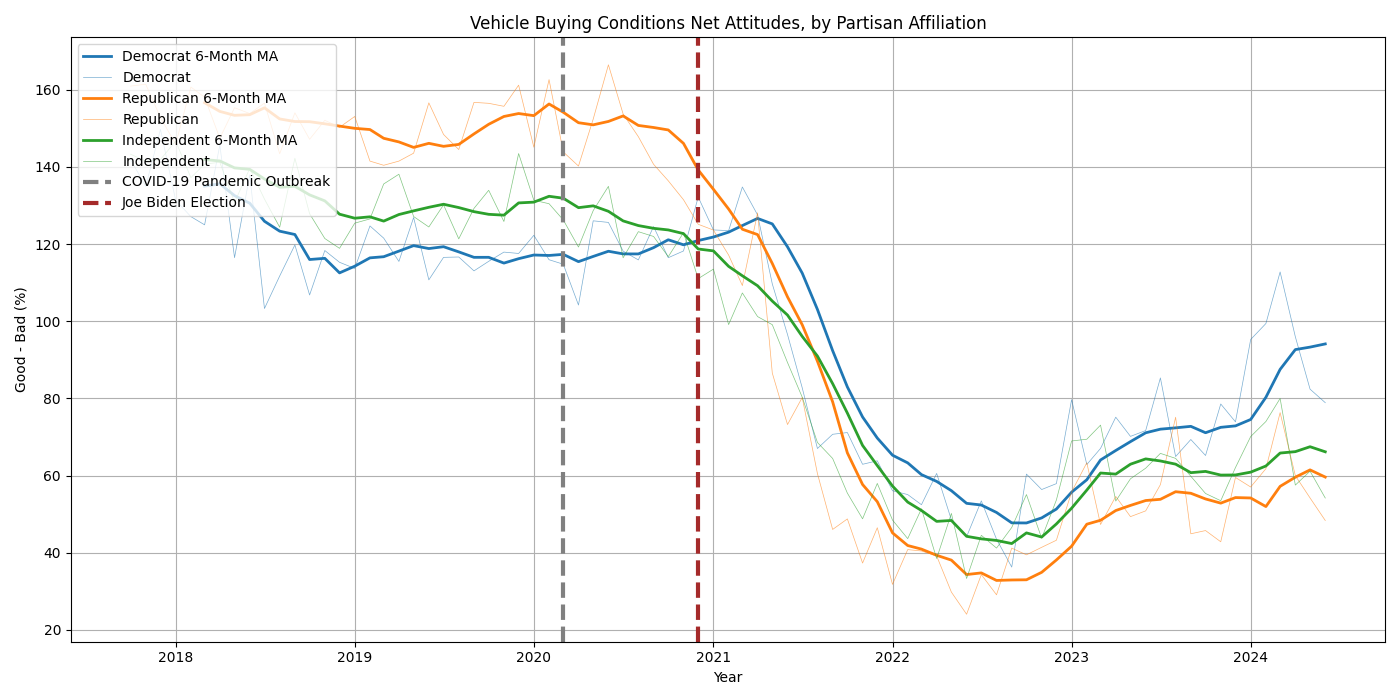
\includegraphics[width=\textwidth]{veh_r_time_series.png}
    %\caption{Vehicle-Buying Conditions}
    \label{fig:veh_time_series}
  \end{subfigure}
  \caption{Reconstructed Net Attitudes by Partisan Affiliation}
  \label{fig:panel}
\end{figure}

Some of these time-series make more sense than others; we saw a volatility in prices--both overall and in gas prices--under President Biden we simply didn't see under President Trump. However, why did voters of every partisan affiliation have their attitudes towards buying a car and house enter a sustained and near-identical decrease nearly exactly when President Biden took office? Then, on the other hand, attitudes towards real household income and predicted positive performance of an investment in the stock market neatly follow the pattern set by the broad economic attitudes sketched above -- with Democrats and Republicans reversing their attitudes upon Biden's inauguration. These descriptive plots suggest some mix of partisan bias and observed economic conditions are shaping attitudes towards the economy. This motivates our  analysis of respondent sensitivity to observed economic changes.

\section{Evaluating Respondent Sensitivity and Bias}
To test whether this is bias or because it was objectively true that the economy was performing better under Trump than Biden, we can match specific questions on the survey to observed economic conditions, as I do in the table below:\footnote{Positive Dummy refers to a dummy variable indicating whether or not a respondent had a positive attitude toward that variable; this simplification of net attitude was necessary because the construction of the net attitude variable is, by necessity, aggregated and not on an individual level. Respondents with either a neutral or negative attitude have a 0 for this outcome variable.}
\begin{table}[ht!]
\begin{threeparttable}
\begin{tabular}{|l|l|l|l|}
\hline
\textbf{Section} 							& \textbf{Question on Survey} 	& \textbf{Outcome} 						& \textbf{Regressor} 		\\ \hline
1-Year Predicted Change in Gas Prices		& GAS1					& GAS								&   National Gas prices \tnote{1} \\ \hline
Home-Buying Conditions		     			& HOM      				& $\text{HOM}_\text{Positive Dummy}$		&   Zillow Home Index\tnote{2}	\\ \hline
Unfavorable News Coverage of Inflation    	& NEWS      				& $\text{NEWSRN\_U\_PRI}_\text{Dummy}$  	&   All-Urban CPI\tnote{3}		\\ \hline
Likelihood of Positive Stock Market Return 	& PSTK     				& PSTK								&   S\&P 500\tnote{4}	 \\ \hline
Real Household Income     				& RINC      				& $\text{RINC}_\text{Positive Dummy}$		&   Real Family Income\tnote{5} \\ \hline
Car-Buying Conditions      					& CAR      				& $\text{VEH}_\text{Positive Dummy}$		&   Used Car CPI\tnote{6} \\ \hline
\end{tabular}
\begin{tablenotes} 
\footnotesize
\item[1] Year-over-year \% change. Source: \href{https://www.eia.gov/dnav/pet/hist/LeafHandler.ashx?n=pet&s=emm_epm0_pte_nus_dpg&f=m}{EIA}
\item[2] Monthly \% change. Source: \href{https://fred.stlouisfed.org/series/USAUCSFRCONDOSMSAMID}{FRED} 
\item[3] Monthly \% change. Source: \href{https://fred.stlouisfed.org/series/CPIAUCSL}{FRED}
\item[4] Year-over-year \% change. Source: \href{https://finance.yahoo.com/quote/\%5EGSPC/}{Yahoo Finance} -- note: I used the closing value for this series at the end of each month.
\item[5] Year-over-year \% change. Source: \href{https://fred.stlouisfed.org/series/A229RX0}{FRED}
\item[6] Monthly \% change. Source: \href{https://fred.stlouisfed.org/series/CUSR0000SETA02}{FRED} 
\end{tablenotes}
\end{threeparttable}
\end{table}

Using these pairs of variable, we estimated this regression using OLS:
\begin{gather}
	 \text{OUTCOME}_{p\text{, }t\text{, }i\text{, }a} = \alpha_{0\text{, }p\text{, }a} + \beta_{1\text{, }p\text{, }a} Z(\text{REGRESSOR}_t) + \epsilon_{p\text{, }t\text{, }i\text{, }a}
\end{gather}
for partisan affiliation $p \in \{\text{Democrat, Republican, Independent}\}$, time $t$, individual $i$, and administration $a \in \{\text{Trump, Biden}\}$. \footnote{Thus, for each economic variable we ran 6 regressions: for 1) Biden-Republican, 2) Biden-Democrat, 3) Biden-Independent, 4) Trump-Republican, 5) Trump-Democrat, and 6) Trump-Independent subsamples.The regressors listed above were also normalized, to reflect that variance in economic conditions were widely different during Biden's vs. Trump's Administration: we normalized the distribution of the percent changes so that a zero value for the regressor would indicate an average percent change during that particular Administration.} Estimates for $\alpha_0$ and $\beta_1$ are plotted below, with 95\% confidence interval bars.

%%%%%%%%%%%%%%%%%%%%%%%%%%%%%%%%%%%%%%%%%%%%%%%%%%%%%%%%%%%%%%%%%%%%%%%%%%%%%%%%%%%%
% plotted regression coefficients
\begin{figure}[ht!]
  \centering
  \begin{subfigure}[b]{0.49\textwidth}
    \centering
    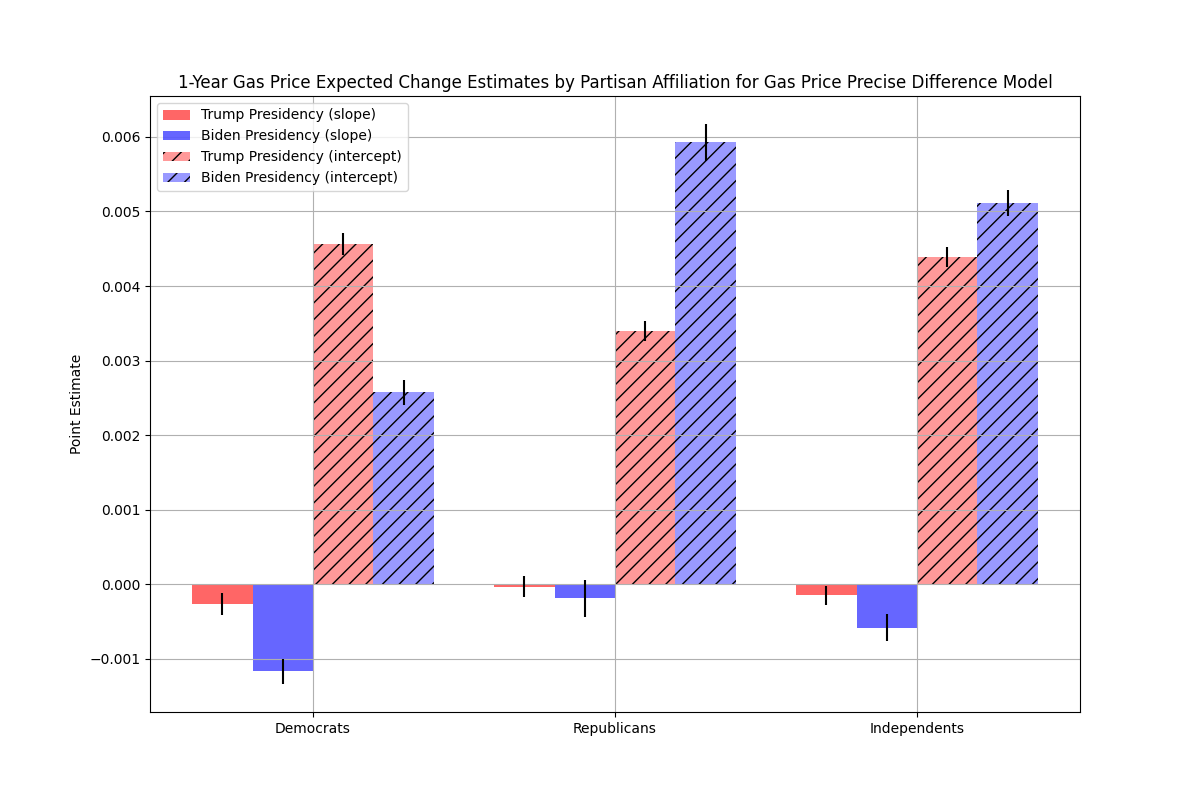
\includegraphics[width=\textwidth]{gas1_model_precise_chg_party_comp.png}
    %\caption{Predicted 1-Year Change in Gas Prices}
    \label{fig:gas1}
  \end{subfigure}
  \begin{subfigure}[b]{0.49\textwidth}
    \centering
    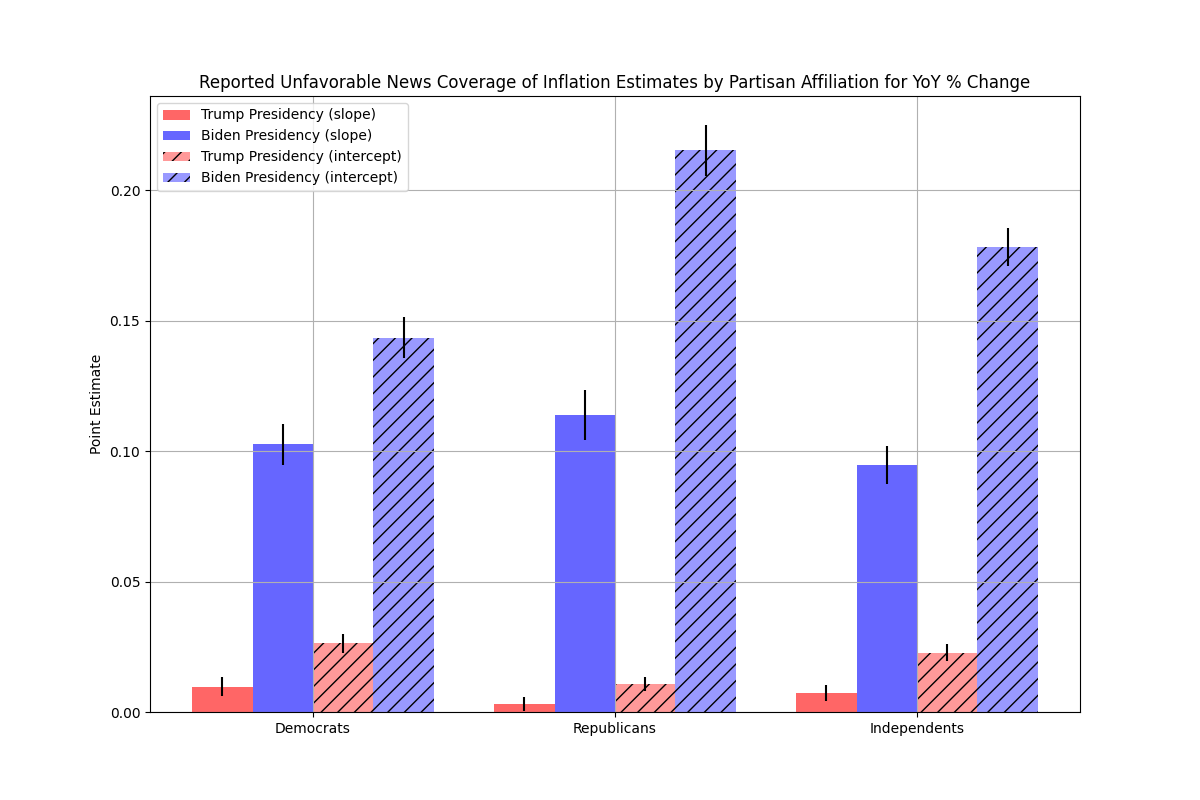
\includegraphics[width=\textwidth]{yoy_news_pri_party_comp_micro.png}
   % \caption{Reported Unfavorable News Coverage of Inflation}
    \label{fig:newsrn}
  \end{subfigure}
   \begin{subfigure}[b]{0.49\textwidth}
    \centering
    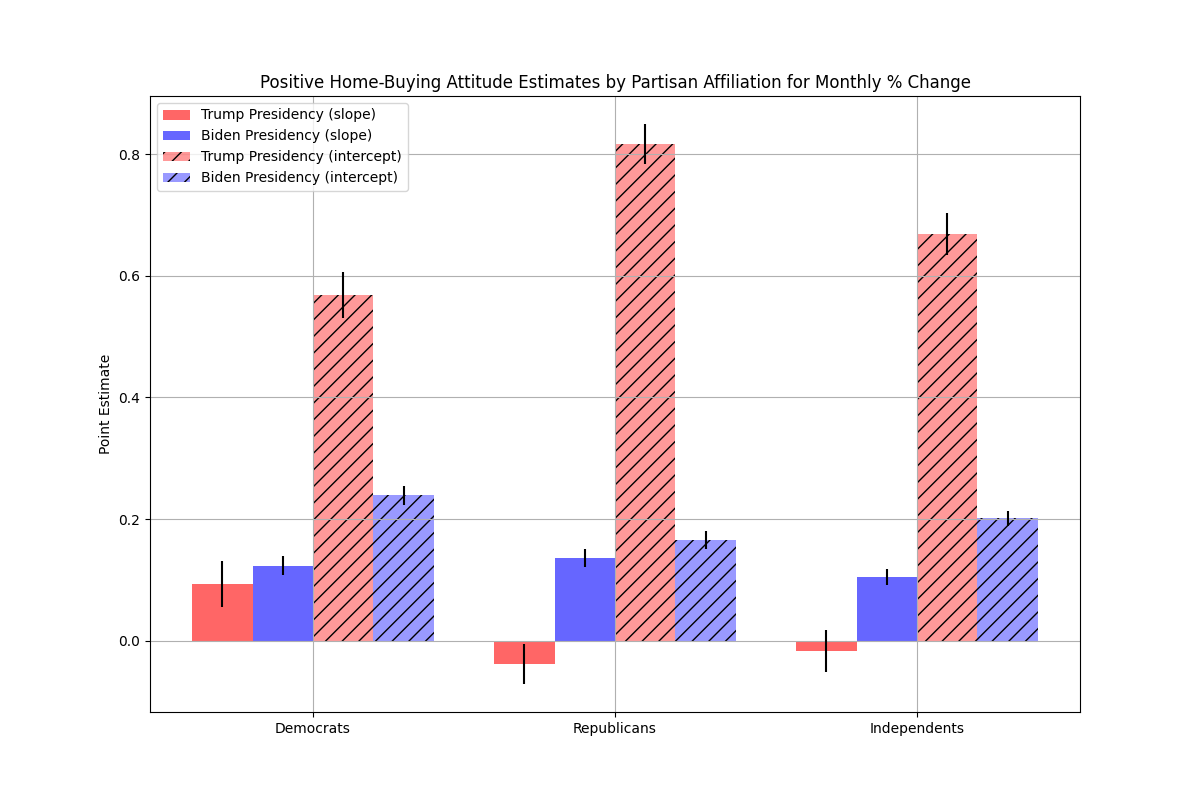
\includegraphics[width=\textwidth]{month_hom_party_comp_micro.png}
    %\caption{Home-Buying Conditions}
    \label{fig:hom}
  \end{subfigure}
   \begin{subfigure}[b]{0.49\textwidth}
    \centering
    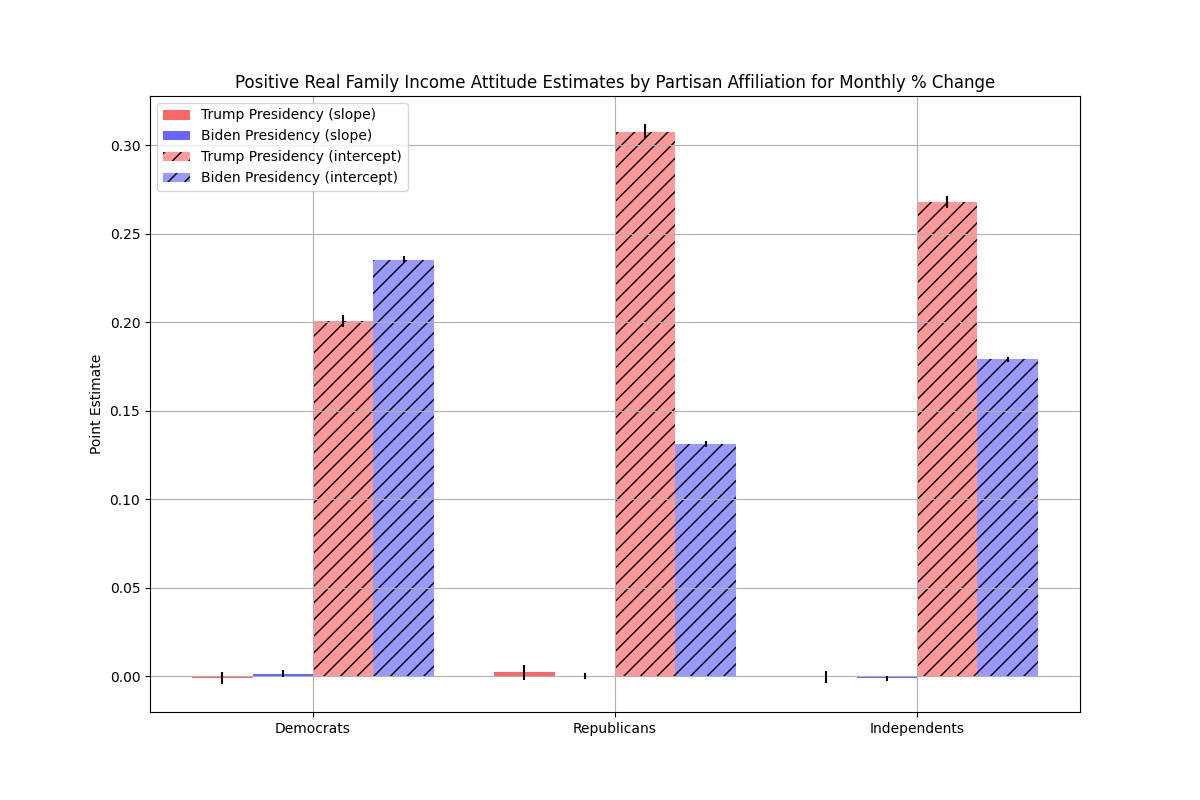
\includegraphics[width=\textwidth]{month_rinc_party_comp_micro.png}
    %\caption{Real Household Income}
    \label{fig:rinc}
  \end{subfigure}
   \begin{subfigure}[b]{0.49\textwidth}
    \centering
    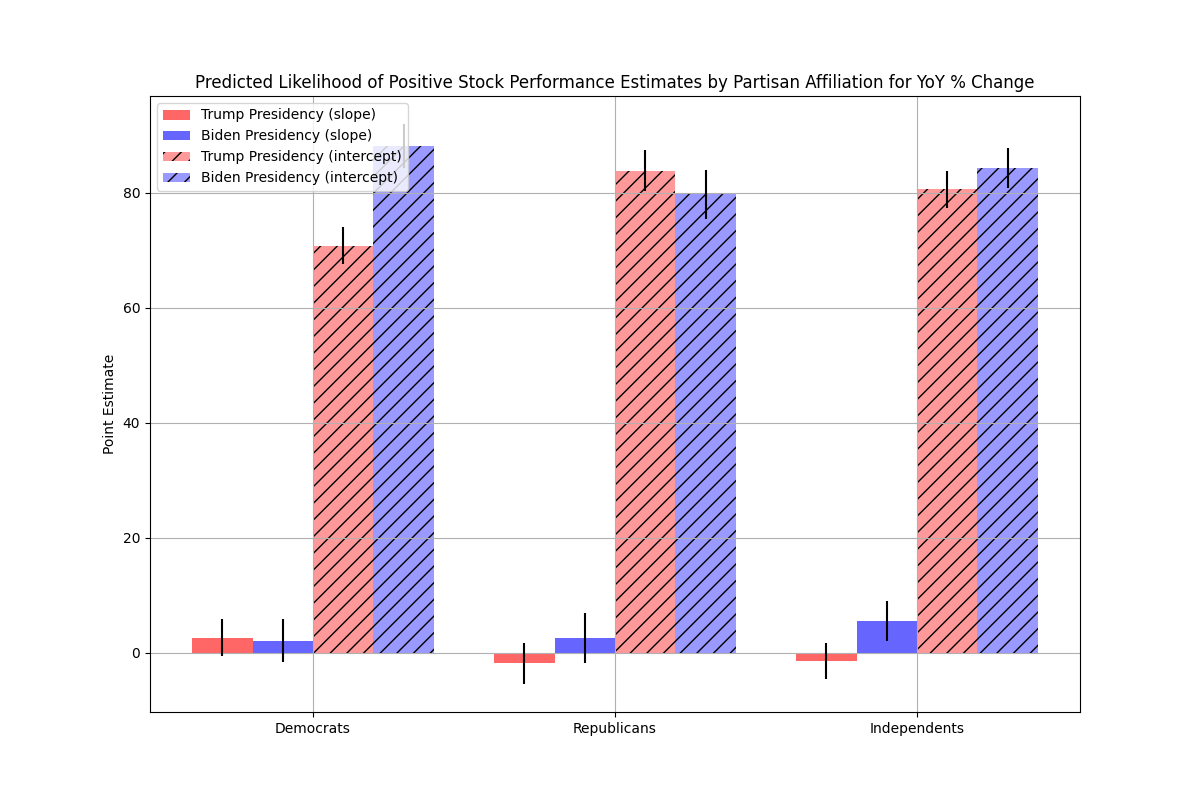
\includegraphics[width=\textwidth]{yoy_pstk_party_comp_micro.png}
    %\caption{Predicted Likelihood of Positive Stock Market Return}
    \label{fig:pstk}
  \end{subfigure}
   \begin{subfigure}[b]{0.49\textwidth}
    \centering
    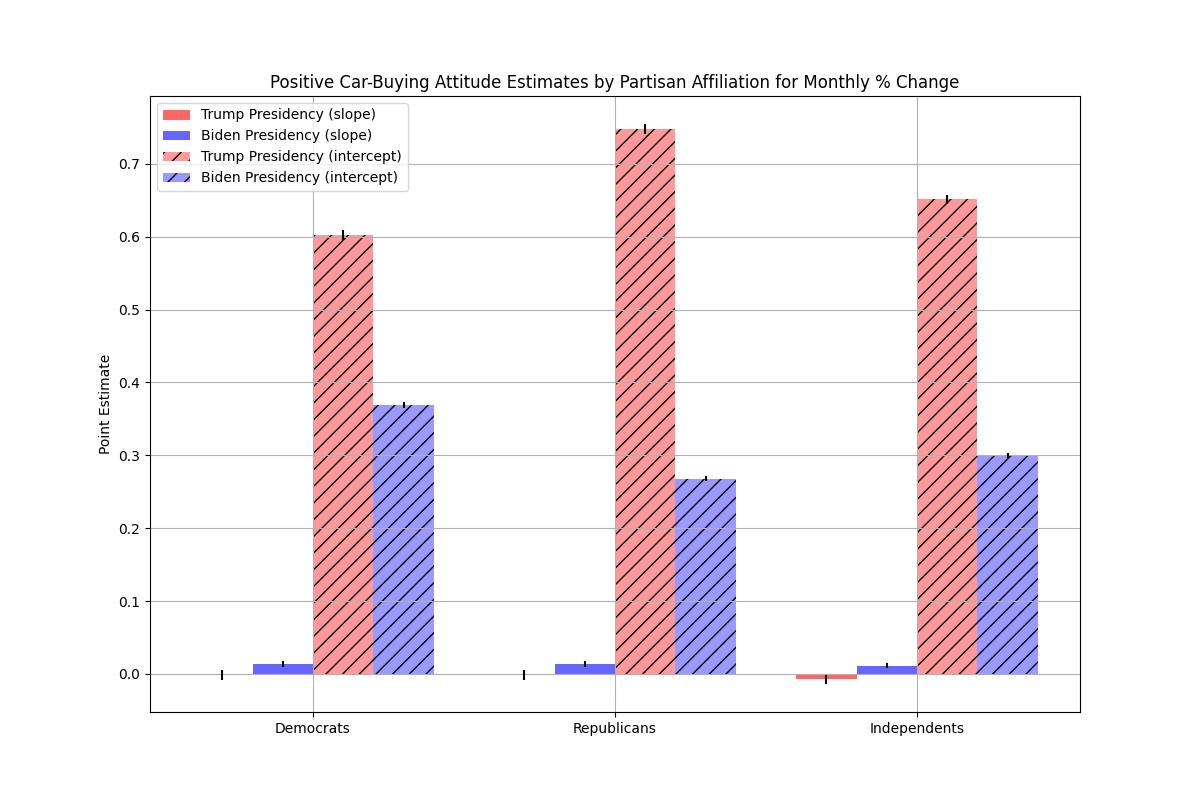
\includegraphics[width=\textwidth]{month_car_party_comp_micro.png}
    %\caption{Vehicle-Buying Conditions}
    \label{fig:veh}
  \end{subfigure}
  \caption{Regression Results by Macroeconomic Variable}
  \label{fig:panel}
\end{figure}

Beginning with gas prices, we find that voters were likelier to predict higher gas price changes under President Biden, even if the percent change from the previous month was exactly average (i.e., the z-score of the change was 0). When this average gas price monthly percent change would occur, Republicans' expected 1-year gas price change would be 4.03 times higher than Democrats', and 1.5 times higher than Independents'. Republicans' expected 5-year gas price change would be 2.28 times higher than Democrats', and 1.16 times higher than Republicans'. 

Reported unfavorable news coverage of inflation had one of the more suggestive descriptive time-series graphs; it appeared that Republicans heard about inflation for longer and more frequently than either Democrats or Independents. Unsurprisingly, there is a significant positive $\beta_1$ coefficient for Democrats, Republicans, and Independents during either the Trump or Biden Administration. The gap seen above appears to be driven by pre-set bias ($\alpha_0$), rather than heightened sensitivity to increasing inflation. For an average change in year-over-year inflation, Republicans were 20.07 times likelier to report unfavorable news coverage of inflation under Biden than Trump, while that figure is 5.46 times for Democrats and 7.82 for Independents.

For the mean monthly percent change in home values, Republicans were 3.09 times likelier to have positive home-buying conditions under President Trump than President Biden. That multiplier is 1.92 for Democrats and 2.43 for Independents. Critically, Republicans and Independents' $\beta_1$ is estimated to be insignificant under Biden--suggesting that for any change larger in magnitude than the mean monthly percent change, Republicans' and Independents' attitudes towards home-buying conditions wouldn't change. On the other hand, Democrats' $\beta_1$ coefficient was significant and positive under Biden as well as Trump, while Republicans' and Independents' estimated $\beta_1$ coefficients were significant and positive during Trump's Administration.

For real household income, none of Democrats, Republicans, nor Independents had a statistically significant $\beta_1$ coefficient--indicating that whether they held positive attitudes towards real family incomes was set by who was President, rather than observed economic conditions. Democrats held a more positive view towards household income under Biden than Trump, while Republicans and Independents were the opposite. However, these findings match earlier work on the \textit{asymmetric} nature of partisan bias. Democrats, for a mean monthly percent change in real family income, were 1.18 times likelier to hold a positive attitude under President Biden than President Trump. Republicans, on the other hand, were 2.35 times likelier to hold a positive attitude under President Trump than President Biden, for a mean monthly percent change in real family incomes. This approximation of partisan bias is nearly twice as large for Republicans than Democrats. 

Interestingly, respondents' predicted likelihood of a positive investment in the stock market after one year had the least evidence of partisan bias, as plotted below. Only Independents had a statistically significant $\beta_1$ coefficient estimate, which was positive during the Biden Administration. This is also the only area where Democrats' partisan bias appears to be greater than Republicans'; for an average year-over-year percentage change in the S\&P500, Democrats appear to be 1.24 times likelier to predict a positive stock market return under Biden than Trump, while Republicans appear to be 1.05 times likelier under Trump than Biden. I suspect that this because this question is less ambiguous than those asking about attitudes towards the economy, and the prediction it is asking respondents to make is easier (since 2016, the S\&P500 has only had 2 years with negative return) than asking about the expected gas price change 5 years from now. 

For used car CPI and car-buying conditions, during the Biden Administration, none of Democrats, Republicans, nor Independents exhibited a statistically significant $\beta_1$ estimated coefficient; however, each group exhibited a positive significant coefficient. Effectively, this suggests that while above-average changes in used car prices would not have affected respondents' attitudes towards car-buying conditions during Trump's Administration, they did during Biden's Administration with a positive correlation. Then, for an average monthly percent change in used car prices, Democrats, Republicans, and Independents were likelier to have a positive attitude during the Trump Administration than Biden Administration. This gap is most magnified for Republicans; Democrats were 1.61 times likelier to have a positive attitude during Trump's Administration than Biden's, while Republicans were 2.75 times likelier. 

\end{document}